\def\mytitle{\textbf{IOT ASSIGNMENT}}
\documentclass[10pt,a4paper]{article}
\usepackage[a4paper,outer=1.5cm,inner=1.5cm,top=2cm,bottom=1.5cm]{geometry}
\usepackage{float}
\usepackage{amsfonts}
\usepackage{titlesec}
\usepackage[utf8]{inputenc}
\usepackage{textgreek}
\usepackage{amsmath}
\usepackage{graphicx} 
\usepackage{enumitem}
\usepackage{tikz}
\usepackage{circuitikz}
\usepackage{karnaugh-map}
\usepackage{tabularx}
\title{\mytitle}
\author{Pavan Srinivas Marri\\marripavan65@gmail.com\\FWC22138 IITH - Future Wireless Communications}
\date{}
\begin{document}
\maketitle
\graphicspath{{./Documents}{./figs}}
\tableofcontents
\section{Problem}
(GATE2021-QP-IN)\\
Q.31 A Boolean function $F$ of three $X$, $Y$ and $Z$ is given as $F(X,Y,Z)=(X' + Y + Z)\cdot(X + Y' + Z')\cdot(X' Y + Z')\cdot(X'Y'Z' + X'YZ' + XYZ')$. Which one of the following is true?
\begin{enumerate}[label=(\alph*)]
    \item $F(X, Y, Z)=(X + Y+ Z')\cdot(X' + Y' + Z')$
    \item $F(X, Y, Z)=(X' + Y)\cdot(X + Y' + Z')$
    \item $F(X, Y, Z)=X'Z' + YZ'$
    \item $F(X, Y, Z)=X'Y'Z + XYZ$
\end{enumerate}
\section{Components}
	\begin{table}[htbp]
		\centering
			\begin{tabularx}{1\textwidth}
			{
				| >{\centering\arraybackslash}X
				| >{\centering\arraybackslash}X
				| >{\centering\arraybackslash}X |}
			\hline
			{\bf Components} & {\bf Value} & {\bf Quantity} \\
			\hline
			Breadboard &  & 1\\
			\hline
			Jumper Wires & & 6 \\
			\hline
			Resistor & 1K$ \Omega $ & 1 \\
			\hline
			LED & & 1\\
			\hline
			Vaman & & 1\\
			\hline
		\end{tabularx}
			\caption{Components}
			\label{table=Components}
		\end{table}
\section{Implementation}
\subsection{Boolean Expression}
	The above equation can be reduced as : \\
	 $\rightarrow (X' + Y + Z)\cdot(X' + Y + Z')\cdot(X + Y' +Z')\cdot(X'Y'Z' + X'YZ' + XYZ')$\\
   	 $\rightarrow(X' + Y)\cdot(X + Y' + Z')\cdot(X'Z' + XYZ')$\\
     	 $\rightarrow(X' + Y)\cdot(X + Y' + Z')\cdot(X'Z' + YZ')$\\
    	 $\rightarrow(X'Y' + X'Z' + YX + YZ')\cdot(X'Z' + YZ')$\\
     	 $\rightarrow X'Y'Z' + X'Z' + X'YZ' + XYZ' + X'YZ' + YZ'$\\
     	 $\rightarrow X'Z' + YZ' + YZ'$\\
      	 $\rightarrow X'Z' + YZ'$\\
    Therefore, the Boolean function $F(X, Y, Z)=(X' + Y)\cdot Z'$
    \subsection{Truth Table}
    \begin{table}[htbp] 
		\centering  
		\begin{tabularx}{0.5\textwidth}
                        {  | >{\centering\arraybackslash}X
                           | >{\centering\arraybackslash}X
                           | >{\centering\arraybackslash}X 
			   | >{\centering\arraybackslash}X |}
                         \hline
			 {\textbf{X}} & {\textbf{Y}} & {\textbf{Z}} & {\textbf{F}} \\
                       \hline 
			0 & 0 & 0 & 1\\   
			\hline  
			0 & 0 & 1 & 0 \\
                       \hline                                                        
			0 & 1 & 0 & 1 \\  
		        \hline   
			0 & 1 & 1 & 0 \\
			\hline
			1 & 0 & 0 & 0 \\
			\hline
			1 & 0 & 1 & 0 \\
			\hline
			1 & 1 & 0 & 1 \\
			\hline
			1 & 1 & 1 & 0 \\
			\hline
		\end{tabularx}
        	        \caption{Truth Table}
			\label{table=truth}
    \end{table}
    \section{Hardware}
    Make the connections between the Breadboard and Vaman borad as follows:
    \begin{enumerate}
    	\item Connect the ground pin(GND) of the Vaman board to the Breadboard's ground rail(-).
 	\item Connect the 5V pin of Vaman board to the beadboard's Positive rail (+).
    	\item Connect the Output pin (Pin 13) of vaman board to one end of resistor on the breadboard and connect LED to the other end of the resistor.
    	\item Give the Power supply to the Vaman board.
    	\item Now Connect the Input pins (Pin 2,3,4) of vaman board to the breadboard's Positive and Negative rails and observe the output.
    	\item Change the connections according to the truth table for different outputs.
    \end{enumerate}
	    \begin{figure}[H]
		    \centering
		    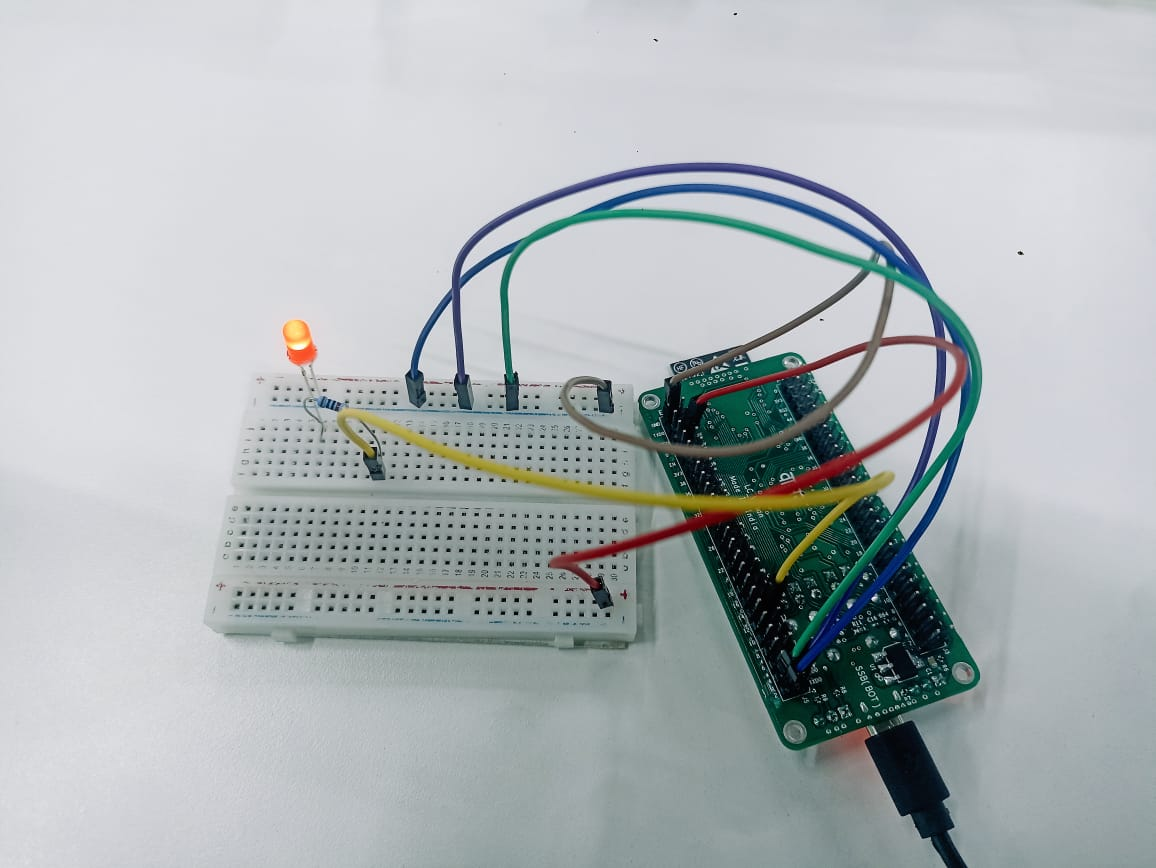
\includegraphics[width=0.3\columnwidth]{iot.jpg}
		    \caption{Connections}
		    \label{fig:connections}
	    \end{figure}
\section{Software}
	Now write the code which is available in the below path and upload it to the Vaman. \\
	\framebox{https://github.com/Pavan2k01/Digital-Design/blob/main/IOT/main.cpp}
\section{Conclusion}
	Hence, We have executed the above code using Vaman according to the given Problem. 
\end{document}
